\subsection{Direct Detection}
\label{DirectDetection}

Direct detection of particle dark matter is possible via their interactions with nuclei in low background terrestrial targets, which appears as one of the most promising techniques. A WIMP elastically scatters off a nucleus in the target material, causing it to recoil and produces an energy deposition of $<$50~keV, which can be transformed into a measurable signal, such as scintillation light, charge, or heat (Fig.~\ref{figDetectionSignals}).

\begin{figure}[!h]
\centering
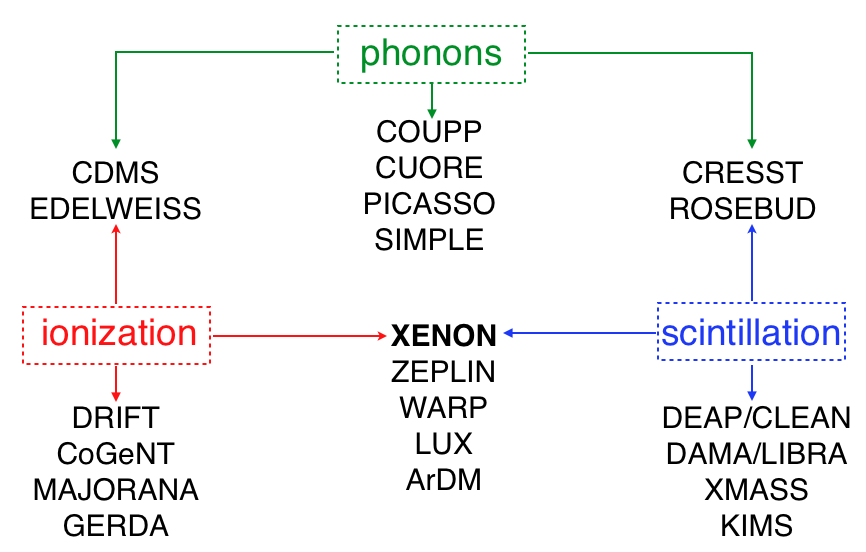
\includegraphics[width=0.6\linewidth]{plots/DarkMatter/DetectionSignals2.png}
\caption[Measurable signals from a WIMP interaction and chart of experiments for direct dark matter detection categorized by measurement technique]{Measurable signals from particle interactions and chart of experiments for direct dark matter detection categorized by measurement technique. The XENON experiment simultaneously measures scintillation and ionization signals, which allows to distinguish between electronic recoil (background) and nuclear recoils (signal) based on their ratio.}
\label{figDetectionSignals}
\end{figure}

The expected exponential nuclear recoil spectrum is featureless, and the shape depends on the mass of the WIMP and the target nucleus. The expected event rate $R$ can be evaluated by taking into account the density and the velocity distributions of WIMPs in the solar neighborhood, and the WIMP-nucleon cross section~\cite{BertoneHooper}:

\begin{equation}
R \approx \sum_{i} N_{i} \cdot n_{\chi} \cdot \sigma_{i\chi},\  \ \text{with}\ \  N_{i} = \frac{m}{A_{i}}\ \ \text{and}\ \ n_{\chi} = \frac{\rho_{\chi}}{M_{\chi}},
\end{equation}
where 
$i$ - index over all nuclei species in the detector, 
$N_{i}$ - number of target nuclei in the detector, 
$m$ - detector mass, 
$A_{i}$ - atomic mass of species $i$, 
$n_{\chi}$ - local WIMP density, 
$\rho_{\chi}$ - WIMP energy density, 
$\sigma_{\chi}$ - the cross section for the WIMP scattering off nuclei of species $i$, averaged over the relative WIMP velocity with respect to the detector.

Results for direct WIMP detection are usually obtained under simplifying assumptions on the galactic dark matter profile, assuming an isothermal profile with a flat rotation curve, a local density of 0.3~GeV/cm$^{2}$, and a Maxwell-Boltzmann velocity distribution. The uncertainties in the parameters lead to an enlargement of the allowed region in the WIMP mass $-$ cross section plane.

The Earth's motion around the Sun results in an annual modulation of the WIMP flux in the order of $<$10\%, thus modulation of the differential event rate over the course of the year, which can be used to separate the (modulated) WIMP signature from an (unmodulated) background. The Earth's speed relative to the galactic rest frame is largest in summer, hence, the WIMP flux with high speeds relative to the detector rest frame is largest in summer~\cite{EarthVelocitySpergel}. Therefore, for larger recoil energies a peak is expected roughly at the beginning of June, and for smaller recoil energies in winter~\cite{ModulationSignal}.

%Also possible is the inelastic WIMP scattering off nuclei~\cite{InelasticScattering_Goodman}, in which the WIMP interacts with orbital electrons, exciting or ionizing them, or with the target nuclei, leaving it in an excited state.
%This signature of this process is a nuclear recoil followed by the emission of a photon. However, the cross section to populate the excited state is a few orders magnitude below the elastic scattering because of phase space effects and smaller overlap of the wave functions~\cite{InelasticScattering_Ellis}. Thus, the backgrounds from natural radioactivity are strong competitors for such signature, and it is rarely used in the direct dark matter detection~\cite{InelasticScattering_DAMA}.

Basic requirements for direct detection detectors are a large target mass, low background, and low energy threshold. For the studies of spin-independent (scalar) coupling, heavy atoms are preferred as target material, as the corresponding cross section increases with the mass of the target nuclei. For spin-dependent (axial-vector) interactions, where the WIMP is expected to couple to unpaired nuclear spins $J$, using heavy targets is no advantage, as the cross section is proportional to $J\cdot$($J$+1) rather than to the number of nuclei, thus increases proportionally to the number of odd-even or even-odd isotopes. 

The first limits on WIMP-nucleon cross-sections have been obtained by the germanium-based double beta decay experiments, such as IGEX and the Heidelberg-Moscow experiment~\cite{FirstLimits_1, FirstLimits_2}, which excluded the first WIMP candidates, such as a heavy Dirac neutrino~\cite{DiracNeutrino} and cosmions~\cite{FirstLimits_Cosmions}. Low energy threshold and high energy resolution make germanium crystals a good target for dark matter searches using the ionization signal~(Fig.~\ref{figDetectionSignals}). 
An example of such an experiment is CoGeNT, which reported a signal~\cite{CoGeNT_LightWIMP} with a modulation~\cite{CoGeNT_modulation}. It could be explained by a WIMP in the mass range below $\sim$10~GeV. However, this explanation has been questioned by Ref.~\cite{Schwetz} and is in conflict with results of other experiments. Other current experiments of this type are GERDA~\cite{GERDA} and MAJORANA~\cite{MAJORANA}. 
However, their primary task is search for the neutrinoless double beta decay of the $^{76}$Ge isotope, a second-order weak process, whose discovery is the only practical way to determine if the neutrino is a Majorana particle~\cite{DoubleBetaGe76}.

Solid scintillation detectors are also being used for dark matter searches by means of light detection. In particular, DAMA is operating a detector based on radio-pure NaI modules, and displayed the annual modulation at a high significance level in the single-hit residual rate which could be due to low mass WIMPs interactions~\cite{DAMA}. Again, this is in conflict with the null-results of other experiments.

The COUPP experiment searches for WIMPs with a bubble chamber, operating a bulk superheated fluid  below the threshold for sensitivity to minimum ionizing particles, and distinguishes electronic and nuclear recoils with a very high efficiency by capturing stereoscopic bubble images and measuring the acoustic signals from bubble nucleation~\cite{COUPP}. PICASSO~\cite{PICASSO} and SIMPLE~\cite{SIMPLE} are examples of superheated droplets detectors, where micro-droplets are suspended in a matrix, which helps to avoid spontaneous bubble formation at the edges.

Some experiments operate at millikelvin temperatures and measure the energy by the collection of phonons simultaneously with the scintillation light, which provides discrimination between nuclear and electronic recoils. One of these experiments is CRESST~\cite{CRESST}, which utilizes Ca$_{2}$WO$_{4}$ crystals with silicon wafers and tungsten superconducting phase transition  thermometers. 
Other experiments, such as CDMS~\cite{CDMS_limit} and EDELWEISS~\cite{EDELWEISS_limit} achieve electronic recoil discrimination by measuring phonons and ionization in germanium crystals.

%The DRIFT experiment is based on the multiwire low pressure gaseous (CS$_{2}$) negative ion time projection chamber, which provides a possibility to reconstruct the ion tracks and deduce the directionality of a WIMP interaction~\cite{DRIFT}.

A very promising technology for WIMP detection are detectors based on noble elements. They are relatively inexpensive, provide easy scalability, require relatively simple cryogenic systems, and have high scintillation and charge yields. XMASS is one of current experiments with the largest target mass ($\sim$800~kg of liquid xenon)~\cite{XMASS}. However, it is a single phase spherical detector, which relies on background reduction only due to good position reconstruction and self-shielding, using only innermost $\sim$100~kg target for dark matter search. In double phase detectors, such as argon based WARP~\cite{WARP} and ArDM~\cite{ArDM}, and xenon-based ZEPLIN~\cite{ZEPLIN} and XENON~\cite{xe100-instrument, EMBG, xe100-run07, xe100-run08}, both scintillation and ionization signals are produced and detected, which allows for background discrimination with a high efficiency. The XENON100 dark matter search detector is the main topic of this thesis, and is covered in detail in the following chapters.



%The first evidence for a positive WIMP signal has been reported by the DAMA experiment in 1997~\cite{DAMA_1997}. However, this result has not been confirmed by 


%The scalar cross-section for spin-independent WIMP-nucleus scattering is given by the following equation~\cite{WIMPnucleusScattering1, WIMPnucleusScattering2}:

%\begin{equation}
%\sigma = F(Q) \frac{4m^{2}_{r}}{\pi} (Z f_{p} + (A-Z) f_{n})^{2},
%\end{equation}
%where $Z$ and $A-Z$ are number of protons and neutrons in the target nucleus, respectively; $f_{p}$ and $f_{n}$ is the WIMP coupling to protons and neutrons; $F(Q)$ - nuclear form factor; $m_{r}$ - reduced mass of the nucleon. 
%Thus, the scattering cross section scales approximately as $A^{2}$, and this gives an advantage of using xenon for WIMP-detection due to the size of the nucleus.
